\chapter{Methodology}
\label{sec:methodology}

This chapter explains what was and will be done within the duration of the whole project. Section \ref{sec:project_overview} describes the overview of the whole project. Section \ref{sec:task_division} elucidates how the tasks were divided among all the involved for this first part of the project, while  \ref{sec:game_gathering} shows how and which games were selected to first test the scripts. Section \ref{sec:packaging} demonstrates the folder structure to create the packages. Section \ref{sec:platform_development} talks about the development of the platform. The chosen tools for the project are specified in Section \ref{sec:tools}

\section{Project Overview}
\label{sec:project_overview}

It has the main goal of creating a platform with all the games developed in the university's courses related to games. The games that will be available must have all their assets and required libraries in a single package that runs in Linux distributions without the need of installing any other package; they also must have a graphical installer for users without technical knowledge.

In order to achieve this goal, the games developed will be cataloged and cloned to a main GitHub organization (whenever possible). Two scripts will be created then, one to build games using SDL 1 and the other for SDL2. The platform itself will be developed while all the other activities take place.

After that, a script will be generated to replicate the packaging system to all of the other games, making the necessary adjustments along the way. The games will be deployed to the website with all of their information and available installers.

The packaging scripts will be integrated and adapted to the platform, so that any student who posts a game will have the installers generated automatically.

\section{Task Division}
\label{sec:task_division}

This project is totally collaborative, it depends and relies on different classes and courses. Because of that, the work was divided among students and teachers, as illustrated in Figure \ref{fig:task_division}.

\begin{figure}[h!]
\centering
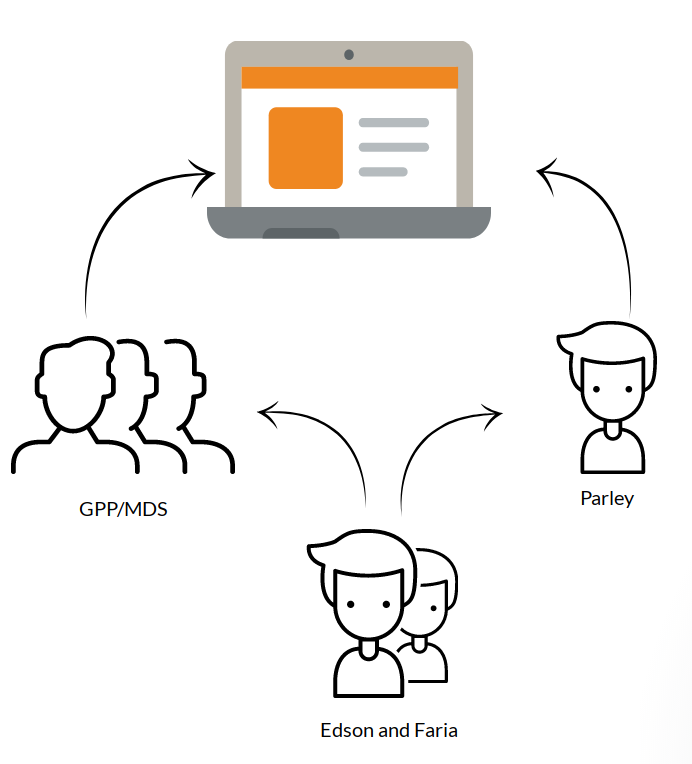
\includegraphics[width=200px,height=\textheight,keepaspectratio]{task_division}
\caption{Task Division}
\label{fig:task_division}
\end{figure}

Professor Edson and Mr. Faria were responsible for first cataloging the existing games. They will remain as helpers in the packaging system and main stakeholders for the team developing the website.

The team \textit{Plataforma de Jogos UnB} from the courses \textit{M\'etodos de Desenvolvimento de Software} (Software Development Methods) and \textit{Gest\~ao de Portfolios e Projetos} (Management of Portfolios and Projects) is in charge of creating the first version of the actual website with some of the features desired. The names of all the members are in the Appendix \ref{sec:members_gpp_mds}.

The scripts creation and their application on the games, their integration with the platform, as well as the evolution and maintenance of the platform after the courses are finished will be my responsibility.


\section{Game Gathering}
\label{sec:game_gathering}

The games selected for this first part of the project were the ones developed in this department, \textit{Faculdade UnB Gama} that is the Gama Campus of the University, since the course \textit{Introdu\c{c}\~ao aos Jogos Eletr\^onicos} (Introduction to Electronic Games) has been created here in the first semester of 2012. Professor Ricardo Jacobi was the first to teach the course, but it wasn't possible to contact him or get the games developed in that term. Professor Edson taught the course after that, until 2016. It has been assumed by Mr. Matheus Faria, since the beginning of this year.

Because this work is being mostly held at FGA, and all the games developed here are compiled and run on Linux distributions, these were selected as first games for the platform. Another reason for this choice is the proximity with the students who created those games.

Professor Edson and Mr. Faria, first contacted the students and asked them to post their codes to GitHub. They cloned them into the \texttt{fgagamedev}\footnote{ \href{https://github.com/fgagamedev}{https://github.com/fgagamedev/} } GitHub organization.


After that, I was responsible for checking the status of the games, gathering information such as which of them compiled, which SDL version they used, which ones had licenses. Table \ref{tab:first_games} shows these initial results.


\begin{table}[h!]
\centering
\caption{Initial status of the selected games}
\label{tab:first_games}
\rowcolors{2}{gray!30}{white}
\begin{tabular}{lcccc}
\toprule
\textbf{Name} & \textbf{Source?} & \textbf{License?} & \textbf{SDL} & \textbf{Compiles?} \\
\midrule
Deadly Wish & y & n & 2 & n \\
Strife of Mythology & y & n & 2 & y \\
Travelling Will & y & n & 2 & y \\
7 Keys & y & MIT & 2 & n \\
Babel & y & GPL 2 & 2 & y \\
Terracota & y & MIT & 2 & n \\
Dauphine & y & n & 2 & n \\
Imagina na Copa & y & n & 2 & y \\
Kays Against the World & y & n & 2 & y \\
Ankhnowledge & y & GPL 2 & 1 & y \\
The Last World War & n & - & - & - \\
Post War & y & n & 1 & y \\
War of the nets & y & GPL 2 & 2 & y \\
Jack the Janitor & y & GPL 3 & 1 & y \\
Drawing Attack & n & - & - & - \\
Earth Attacks & n & - & - & - \\
Emperor vs Aliens & y & n & 1 & y \\
Ninja Siege & y & GPL 2 & 1 & y \\
Space monkeys & y & GPL 2 & 1 & n \\
Tacape & n & - & - & - \\
\bottomrule
\end{tabular}
\end{table}

Out of 20 games created in \textit{Introdu\c{c}\~ao aos Jogos Eletr\^onicos} while Professor Edson taught it, 4 didn't have a known repository and 8 didn't have a license that allowed us to change them at that time. Mr. Faria and I were responsible for finding unknown games and getting the missing licenses. As result of this task, \textit{The Last World War} was added and 5 other had licenses acquired as shown in Table \ref{tab:final_games}.

\begin{table}[h!]
\centering
\caption{Game status after contacting developers}
\label{tab:final_games}
\rowcolors{2}{gray!30}{white}
\begin{tabular}{lccc}
\toprule
\textbf{} & \multicolumn{1}{l}{\textbf{License}} & \multicolumn{1}{l}{\textbf{SDL}} & \multicolumn{1}{l}{\textbf{Compiles}} \\
\midrule
Deadly Wish & GPL 3 & 2 & n \\
Strife of Mythology & GPL 2 & 2 & y \\
Travelling Will & MIT & 2 & y \\
7 Keys & MIT & 2 & n \\
Babel & GPL 2 & 2 & y \\
Terracota & MIT & 2 & n \\
Dauphine & MIT & 2 & n \\
Imagina na Copa & MIT & 2 & y \\
Kays Against the World & n & 2 & y \\
Ankhnowledge & GPL 2 & 1 & y \\
The Last World War & n & 1 & y \\
Post War & MIT & 1 & y \\
War of the nets & GPL 2 & 2 & y \\
Jack the Janitor & GPL 3 & 1 & y \\
Emperor vs Aliens & n & 1 & y \\
Ninja Siege & GPL 2 & 1 & y \\
Space monkeys & GPL 2 & 1 & n \\
\bottomrule
\end{tabular}
\end{table}


\section{Packaging}
\label{sec:packaging}

The template for packaging was created by professor Edson is based on two main directives, modularisation and platform independence. The first one is related to dividing the directories by topic, meaning that, each folder will be responsible for one thing and all the files inside of them should be related to that specific thing. The second directive, platform independence, is to make the development for multiple platforms easy. Each directory will have a division for each of the platforms.

To achieve the template modularision, professor Edson decided to use a folder structure that would be easy to understand to anyone familiar with GNU/Linux FHS, with a few additions. Apart from the original directories in the repository, he added the folders \texttt{bin}, \texttt{dist}, \texttt{lib} and \texttt{scripts}. This structure is represented in Figure \ref{fig:folder_structure}

\begin{itemize}
\item \texttt{scripts} this is where the scripts to build, package and distribute the binaries for all the platforms will live. It also has a subdirecoty called \texttt{utils} that holds some specific platform scripts, like generating each installer, or gather information about the host OS;
\item \texttt{lib} All the third-party libaries should live here. The scripts to build the code are already set to look for libs inside this directory, being each subdirectory a dependency;
\item \texttt{dist} This contains the files needed to generate the packages for each platform;
\item \texttt{bin} has all needed libraries and the game executable.

\end{itemize}

\begin{figure}[h!]
\centering
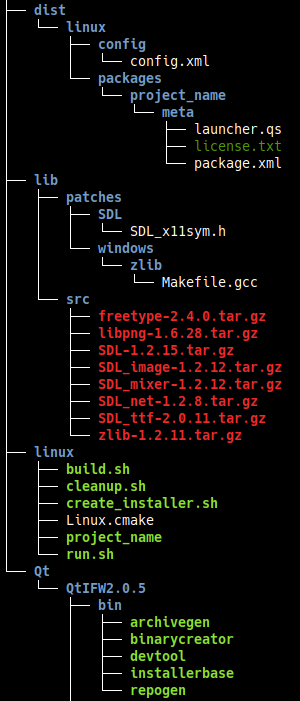
\includegraphics[scale=0.7]{folder_structure}
\caption{Folder tree}
\label{fig:folder_structure}
\end{figure}

The second directive was met by dividing some of the directories into platform limited directories, making the code that lives there accessible only when running on that individual platform. Any file outside the platform directory is considered generic, and can be used for any Operating System. For example, when running on Windows, the compiler would only access generic files and Windows specific ones, like \texttt{dlls}. The same thing happens for macOS and GNU/Linux systems. This division is represented inside the \texttt{lib} directory in Figure \ref{fig:folder_structure_lib}.

\begin{figure}[h!]
\centering
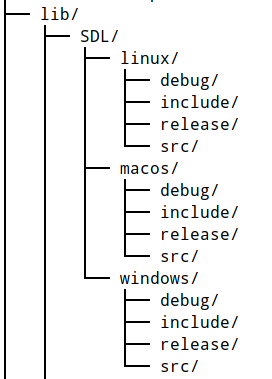
\includegraphics[scale=0.7]{folder_structure_lib}
\caption{Platform and library division}
\label{fig:folder_structure_lib}
\end{figure}

As also seen in Figure \ref{fig:folder_structure_lib}, inside each platform folder (only for libraries) there is yet another division to make sure the template can generate different versions of the program for \texttt{debug} and \texttt{release}. The binaries that live on \texttt{release} are stripped of all debug symbols, resulting in smaller versions of those dependencies. Library headers go inside \texttt{include} and a compressed file with the source goes inside \texttt{src}.


Another main concern in the template creation was making a small dependency chain, using as many native tools as possible. For example, the chosen compiler was GCC for Linux, Visual Studio for Windows and CLang for macOS. To control the generation of executables, GNU Make was chosen. The scripts were all written in Bash (native for macOS and Linux).


\section{Platform Development}
\label{sec:platform_development}

The first version of the platform was developed using mixed development methods. During the first half of the semester, the Rational Unified Process  and the PMBOK were used. For the next part, Scrum and XP were chosen. This choice of development framework is because of how the courses are divided.

Throughout the RUP part of the development, the team created several documents to aid the development cycle, such as, vision, architecture document, class diagram, use case diagram, use case specification, test case specification.

These documents helped the team to understand the system requirements and how they should be implemented as seen in Figure \ref{fig:class_diagram}. The most experienced members also helped the others to learn the technologies to develop the website.


\begin{figure}[h!]
\centering
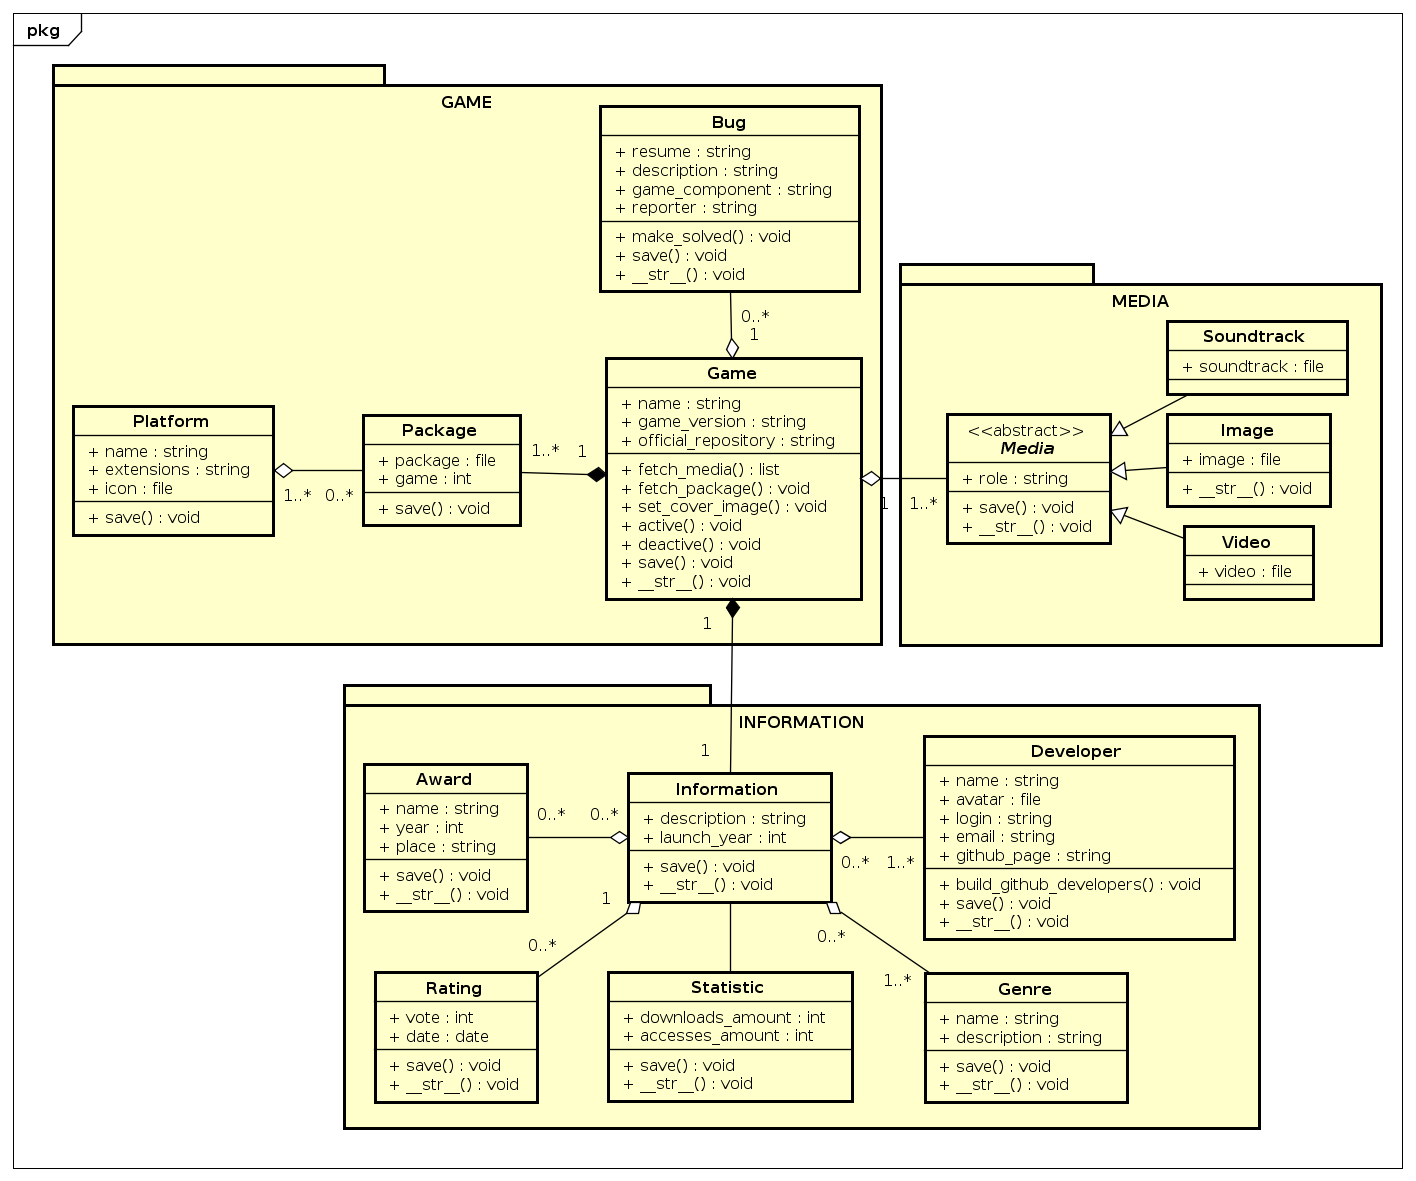
\includegraphics[width=\textwidth,height=\textheight,keepaspectratio]{class_diagram}
\caption{Class Diagram of the Platform \cite{plataforma2017arquitetura}}
\label{fig:class_diagram}
\end{figure}

As the second part of the development started, they had to work on a totally different mindset, with new roles and documents needed. Instead of having managers, the team had now Scrum Master, Product Owner and the Developing team \cite{agile422017}. A Scrum Master is the responsible for protecting the team, making sure knowledge is being shared and Scrum is being followed \cite{scrumalliance2017}. It's important to notice that this is not equivalent to a traditional manager, that usually only bosses around the team, not caring about the people.

Product Owner is the one who will say the product value, sets the priorities and decides what need be done \cite{agile422017}. They must assure the work meets their expectations without controlling the development team \cite{scrumalliance2017}. The Development Team are the people who will actually do the work, they don't have a manager, they act collectively and decide how they will achieve what has to be done \cite{scrumalliance2017}.

For the next semester, I'll be the responsible the development and maintenance of the platform. It's intended to use Agile Practices for the rest of the development, whenever possible, but that won't be a requirement, since I'll be mostly working alone on these tasks. A more detailed account of what will be done can be found in Chapter \ref{sec:future_work}.


\section{Tools}
\label{sec:tools}

CMake was the chosen framework for generating the packages. It's suppose to help developers creating applications that run in several platforms, like Linux, Mac and Windows. It offers a lot options for that, like cross compilation and compilation directed to each of them. It is distributed under OSI-approved BSD 3-clause License and the minimum required version is 2.8.

For the graphical installer, Qt Installer Framework has been selected. It is easy to use and offers a nice GUI with all the necessary steps for installing a package, like license agreement and path choice. This framework is distributed under LGPLv3 license and the version being used is 2.0.5.

For the website development, Django was picked because of the previous knowledge the group had with it. To make the front end of the application, Facebook's React was chosen for the flexibility it gives to the user interface. They are both very scalable, have a big support on the community and are released under the BSD 3-clause license. The versions being used are the last ones at the beginning of the project, namely, 1.11.1, for Django, and 15.5.4, for React.

Python was the language for the packaging script because it must integrate with the Django webapp and its powerful easy to use API. It will also be the language for any other needed scripts. The least required version is 3.4, and it's licensed under an OSI-approved open source license.

To develop the scripts, a virtual machine running Debian Jessie was used. The VM was powered by Vagrant, version 1.9, that allows easy environment virtualization. It also enables a developer to test in several operating systems, which is required for the nature of this project. The computer hosting the script and used to its development has an Intel Core i5-6200U 2.3 GHz processor. It also has 8 GB of RAM and an NVIDIA GeForce 940M graphic processor.
